% Options for packages loaded elsewhere
\PassOptionsToPackage{unicode}{hyperref}
\PassOptionsToPackage{hyphens}{url}
%
\documentclass[
  12pt,
]{article}
\usepackage{lmodern}
\usepackage{amssymb,amsmath}
\usepackage{ifxetex,ifluatex}
\ifnum 0\ifxetex 1\fi\ifluatex 1\fi=0 % if pdftex
  \usepackage[T1]{fontenc}
  \usepackage[utf8]{inputenc}
  \usepackage{textcomp} % provide euro and other symbols
\else % if luatex or xetex
  \usepackage{unicode-math}
  \defaultfontfeatures{Scale=MatchLowercase}
  \defaultfontfeatures[\rmfamily]{Ligatures=TeX,Scale=1}
\fi
% Use upquote if available, for straight quotes in verbatim environments
\IfFileExists{upquote.sty}{\usepackage{upquote}}{}
\IfFileExists{microtype.sty}{% use microtype if available
  \usepackage[]{microtype}
  \UseMicrotypeSet[protrusion]{basicmath} % disable protrusion for tt fonts
}{}
\usepackage{xcolor}
\IfFileExists{xurl.sty}{\usepackage{xurl}}{} % add URL line breaks if available
\IfFileExists{bookmark.sty}{\usepackage{bookmark}}{\usepackage{hyperref}}
\hypersetup{
  pdftitle={Spotify Clarifies},
  pdfauthor={Britney Brown, Harrison DiStefano, Greg Eastman; Lisa Kaunitz, Tianyang Liu, Jeremy Weidner},
  hidelinks,
  pdfcreator={LaTeX via pandoc}}
\urlstyle{same} % disable monospaced font for URLs
\usepackage[left=12mm, right=12mm, top=15mm, bottom=15mm]{geometry}
\usepackage{graphicx}
\makeatletter
\def\maxwidth{\ifdim\Gin@nat@width>\linewidth\linewidth\else\Gin@nat@width\fi}
\def\maxheight{\ifdim\Gin@nat@height>\textheight\textheight\else\Gin@nat@height\fi}
\makeatother
% Scale images if necessary, so that they will not overflow the page
% margins by default, and it is still possible to overwrite the defaults
% using explicit options in \includegraphics[width, height, ...]{}
\setkeys{Gin}{width=\maxwidth,height=\maxheight,keepaspectratio}
% Set default figure placement to htbp
\makeatletter
\def\fps@figure{htbp}
\makeatother
\setlength{\emergencystretch}{3em} % prevent overfull lines
\providecommand{\tightlist}{%
  \setlength{\itemsep}{0pt}\setlength{\parskip}{0pt}}
\setcounter{secnumdepth}{-\maxdimen} % remove section numbering
\usepackage{indentfirst} \usepackage{background} \usepackage{float} \backgroundsetup{ scale=1, color=black, angle=0, pages=all, contents={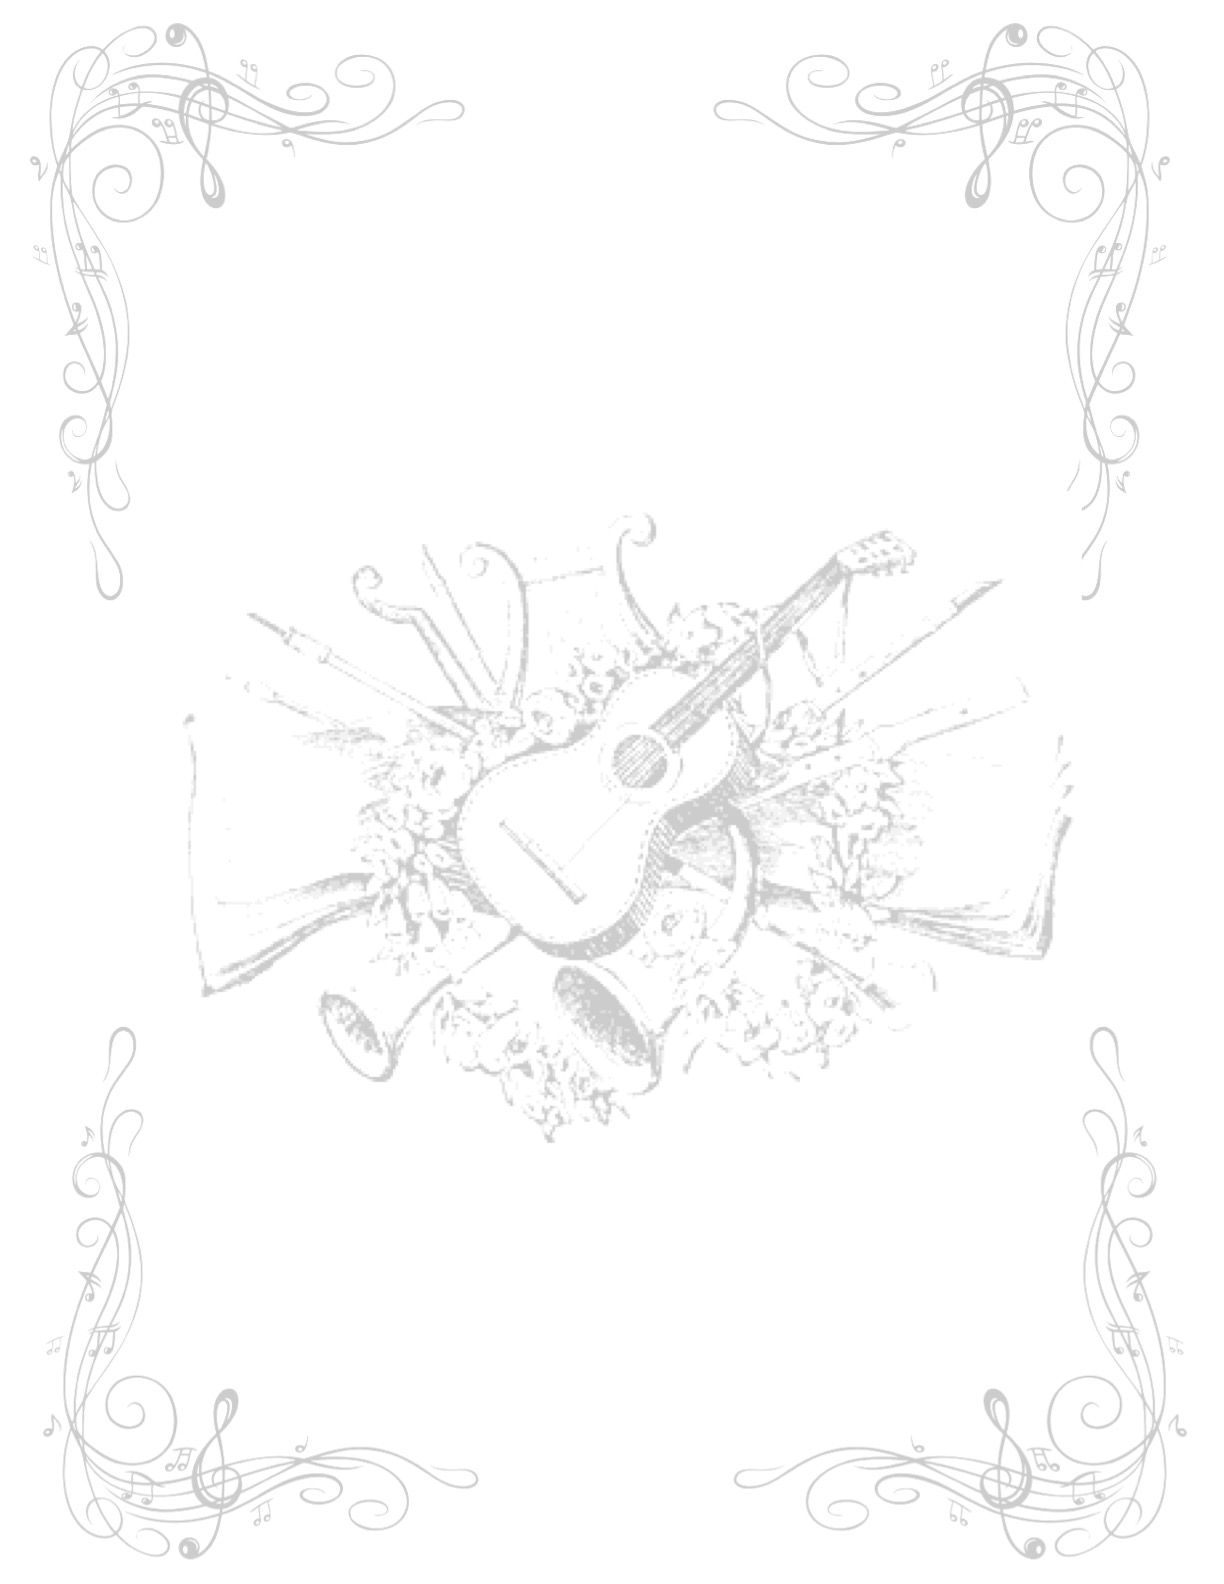
\includegraphics[width=22cm,height=52cm]{music_graphic.jpg}} }

\title{Spotify Clarifies}
\usepackage{etoolbox}
\makeatletter
\providecommand{\subtitle}[1]{% add subtitle to \maketitle
  \apptocmd{\@title}{\par {\large #1 \par}}{}{}
}
\makeatother
\subtitle{An Analysis of Music Popularity over Time}
\author{Britney Brown, Harrison DiStefano, Greg Eastman \and Lisa
Kaunitz, Tianyang Liu, Jeremy Weidner}
\date{06/04/2021}

\begin{document}
\maketitle

Music has been an integral part of our culture since well before the
invention of the computer. Lately we have seen digital music take the
industry by storm, which for the first time in musical history gives us
the ability to analyze the quantifiable components of the music we all
enjoy. Popular music has evolved significantly over the last fifty years
from songs like the Beatles' ``I Want to Hold Your Hand'' to Taylor
Swift's ``Shake it Off.'' Although we recognize a shift here, what can
the data behind these songs tell us about trends in the music industry?

Through our analysis, we revealed four \textbf{Key Insights}:

\begin{itemize}
\item
  We discovered two important themes that span across all time: emotions
  and relationships. Regardless of societal evolution, expressing our
  emotions towards the people we care for seems to be a constant force.
\item
  We also found that people tend to prefer sad, depressing songs more in
  recent years. A quick scan of current events through recent years will
  probably make this one of our less surprising findings.
\item
  In order for a song to be ``danceable'', there should be some acoustic
  presence, high valence (positive sounds), a slightly above average
  loudness, and finally to avoid too much instrumentalness.
\item
  In the last 20 years, tracks have consistently maintained
  approximately nine sections. This steady approach to song structure
  highly suggests the introduction of a breakthrough algorithmic
  approach towards song creation in order to increase success potential.
\end{itemize}

\vspace{8pt}

Using data from Spotify, we analyzed song construction to see what makes
particular songs timeless and others forgettable. We looked at the
overall trends found in songs over time and analyzed qualities that hit
tracks seem to have in common. Our overall goal was to get a better
interpretation of musical trends and a greater understanding of the
modern music world.

\vspace{8pt}

Data available to us in this analysis was a wide range of descriptive
statistics about a given selection of tracks including danceability,
energy, key, loudness, tempo, decade and whether or not the track was a
``hit'' amongst other variables.

\vspace{8pt}

Further in the analysis we take a look at how danceability relates to
other song attributes such as acousticness, instrumentalness, loudness
and valence to determine what features make a song a bop rather than a
ballad.

\vspace{8pt}

Finally, we see how the decades stack up against each other by comparing
song duration, major and minor mode percentages, and other variable
changes in music across decades.

\end{document}
